\chapter{Organización de los datos en un SGBD Relacional}


\begin{figure}[H]
  \center
  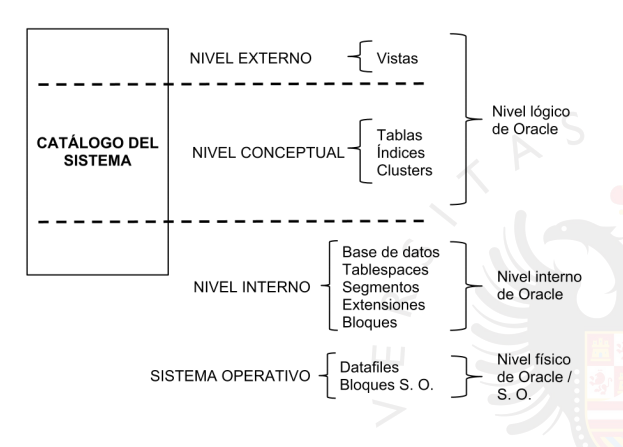
\includegraphics[scale=0.4]{img/8.png}
  \caption{De qué vamos a hablar}
\end{figure}

\section{Catálogo}

En un modelo relacional, toda la información que hay dentro del sistema se almacena en estructuras relacionales, es decir, se almacena información sobre las tablas, en una tabla. Desde esa perspectiva, llamamos \textbf{diccionario de datos} o el \textbf{catálogo} al conjunto de estructuras para almacenar información sobre los datos. Esos datos sobre los datos, se llaman normalmente \textbf{metadatos}.

El catálogo de compone de una serie de objetos entre los que se encuentran:
\begin{itemize}
\item Tablas (atributos, tipos de datos, restricciones, propietario, etc)
\item Vistas (nombre, consulta asociada, propietario, etc)
\item Índices (nombre, tabla, atributos, tipo, propietario, etc)
\item $\cdots$
\end{itemize}
Pero no solo eso, también contiene:
\begin{itemize}
\item Espacio y estructuras de nivel interno
\item Integridad de objetos
\item Usuarios
\item Privilegios y roles
\item Información para auditoría
\item Información sobre la BD (tablespaces, datafiles, etc).
\end{itemize}

Esto significa que el catálogo almacena información sobre \textbf{todos} los niveles de la base datos. ¿Cómo se organiza toda esta información? Como son tablas e índices, se consultan y se manejan como las estructuras de datos estudiadas en los dos capítulos anteriores. Los objetos se almacenan en un tablespace llamado \textbf{SYSTEM}. La información se almacena en:
\begin{itemize}
\item Tablas: denominadas tablas base, sólo accesibles al SGBD y el usuario \textit{sys}, aunque no se recomienda accederlas directamente. El usuario \textit{sys} tiene acceso a ellas porque necesita crearlas al principio de la base de datos. Para consultarlas, se recomienda el uso del siguiente punto.
\item Vistas: sirven para el acceso simple, selectivo y personalizado de la infromación de las tablas base y están accesibles a cualquier usuario (dependiendo de sus permisos).
\end{itemize}

En la organización del catálogo, los nombres de los objetos son importantes:
\begin{itemize}
\item Si comienza por \textbf{USER\_...}: determina que la vista contiene información sobre los objetos del usuario que ejecuta la consulta.
\item Si comienza por \textbf{ALL\_...}: determina que la vista contiene información sobre todos los objetos \textbf{accesibles} para el usuario que ejecuta la consulta (incluya le información de \textit{USER\_...}
\item Si comienza por \textbf{DBA\_...}: determina que la vista consulta la tabla de catálogo tal y como está almacenada (solo el usuario sys y otros con permiso pueden hacerlo).
\end{itemize}

Mantener toda esta estructura sobre la información de la base de datos tiene varias utilidades:
\begin{itemize}
\item Organizar la información de la manera más eficiente posible, y dado que la hemos diseñado con una estructura que permite almacenar información de los usuarios de forma eficiente, ¿por qué no usar esa misma estructura para almecenar la información del sistema?
\item Al tener la información organizada, es mucho más sencillo mantenerla actualizada. Basicamente, todas las operaciones que realizamos sobre el sistema tienen un efecto sobre el catálogo que se actualiza de forma rápida.
\item Además, tener la información almacenada permite conocer mucha información  sobre los tres niveles de la base de datos (externo, conceptual y físico). 
\end{itemize}

\begin{example}
Supongamos la siguiente sentencia sql:
\begin{lstlisting}[ language=SQL,
                    deletekeywords={IDENTITY},
                    deletekeywords={[2]INT},
                    morekeywords={clustered},
                    framesep=8pt,
                    xleftmargin=40pt,
                    framexleftmargin=40pt,
                    frame=tb,
                    framerule=0pt ]
CREATE TABLE CARD (
    CARDID VARCHAR2(20) CONSTRAINT CARD_CARDID_PK PRIMARY KEY,
    CARDNAME VARCHAR2(30) CONSTRAINT CARD_CARNAME_NOTNULL NOT NULL,
    ACCOUNTING VARCHAR2(20)
      CONSTRAINT CARD_ACCOUNTNO_NOTNULL NOT NULL,
      CONSTRAINT CARD_ACCOUNTNO_FK REFERENCES ACCOUNT,
	EXPDATE DATE CONSTRAINT CARD_EXPDATE_NOTNULL NOT NULL,
	DAYLYLIMIT NUMBER(4)
	  CONSTRAINT CARD_DAILYLIMIT_NOTNULL NOT NULL
	  CONSTRAINT CARD_DAILYLIMIT_POSSITIVE CHECK DAILYLIMIT>=0,
	LASTLIMIT NUMBER(6,2)
	  CONSTRAINT CARD_LASTLIMIT_NOTNULL NOT NULL
	  CONSTRAINT CARD_LASTLIMIT_POSSITIVE CHECK LASTLIMIT >=0
	  AND
	  CONSTRAINT CARD_LAST_LIMIT_LESSTHANDAILY
	    CHECK LASTLIMIT <= DAILYLIMIT
);
\end{lstlisting}

Lo primero que se crea es el objeto \textit{CARD} (linea 1). Hay que tener en cuenta que toda tabla de la BD, antes de ser una tabla, es un objeto, es decir, primero tenemos que almacenar información sobre el objeto en sí, y después almacenamos información del objeto visto como tabla. Lo que significa que, después de ejecutar la línea 1, podemos consultar información sobre este objeto en dos tablas diferentes:
\begin{itemize}
\item Vista \textit{USER\_OBJECTS}: que nos dará información de la tabla vista como un objeto.
\item Vista \textit{USER\_TABLES}: que nos dará información de la tabla vista como tabla. 
\end{itemize}
Luego nos encontramos una seria de columnas o atributos (líneas 2,3,4,7,8 y 11) sobre los que también se va a almacenar información. Esta información se va a 
guardar en \textit{USER\_TAB\_COLUMNS}. Sin embargo, como para cada una de las columnas (o atributos) podemos poner una serie de restricciones, incluso más de una, eso nos impide que podamos guardar la información de las restricciones en la misma tabla que guardamos la información de la columna. La información sobre las restricciones se va a guardar en la vista \textit{USER\_TAB\_CONSTRAINTS}.
\end{example}

\section{Estructura interna}

Hablemos ahora de los elementos de la estructura interna de la BD. Lo habitual, es que exista un fichero conteniéndolo 'todo', es decir, ficheros muy grandes con mucha información. De forma que si en un fichero metemos información sobre muchos usuarios y habitualmente los usurios consultan su propia información, es interesante que la información de un usuario esté cercana entre sí. Es decir, organizamos la información del fichero en bloques de forma eficiente para la consulta. Recordemos que a nivel del SO y del sistema de ficheros solo hay bloques y ficheros, pero al nivel físico de Oracle, hay: tablespaces, segmentos, extensiones y bloques. Esos elementos siguen presentan la siguiente jerarquía:

\begin{figure}[H]
  \center
  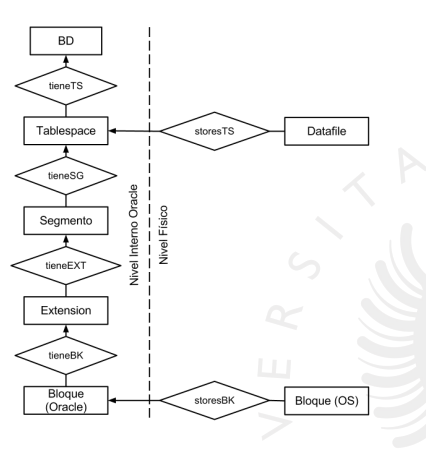
\includegraphics[scale=0.5]{img/9.png}
\end{figure}

Esa imagen que leerla como: la BD tiene \textit{tablespaces} (TS), que se repsentan en el nivel físico mediante \textit{datafiles}. Los \textit{tablespaces} además contienen \textit{segmentos}, y cada segmento almacena una serie \textit{extensiones}, que a su vez tienen \textit{bloques de Oracle} (no del SO). Por último, los bloques de Oracle son almacenados usando bloques del SO.

\subsection{Tablespaces}
\begin{lstlisting}[ language=SQL,
                    deletekeywords={IDENTITY},
                    deletekeywords={[2]INT},
                    morekeywords={clustered},
                    framesep=8pt,
                    xleftmargin=40pt,
                    framexleftmargin=40pt,
                    frame=tb,
                    framerule=0pt ]
CREATE TABLESPACE users DATAFILE "c:\oracle\oradata\users01.dbf" SIZE 20M;
\end{lstlisting}
\begin{figure}[H]
  \center
  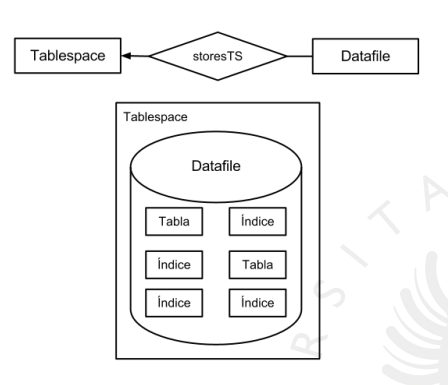
\includegraphics[scale=0.4]{img/10.png}
\end{figure}

Un tablespace se compone de una serie de datafiles, esto quiere decir que cuando se crea uno, hay que especificarle al menos un datafile que se creará dentro de los directorios del SGBD para manejarlo.

Puede darse el caso de que la información dentro de ese tablespace crezca tanto que se sature. En ese caso, lo único que tenemos que hacer es añadirle otro datafile más:

\begin{lstlisting}[ language=SQL,
                    deletekeywords={IDENTITY},
                    deletekeywords={[2]INT},
                    morekeywords={clustered},
                    framesep=8pt,
                    xleftmargin=40pt,
                    framexleftmargin=40pt,
                    frame=tb,
                    framerule=0pt ]
ALTER TABLESPACE users ADD DATAFILE "c:\oracle\oradata\users02.dbf" SIZE 20M;
\end{lstlisting}
\begin{figure}[H]
  \center
  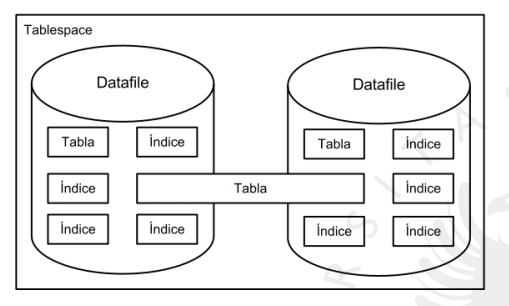
\includegraphics[scale=0.4]{img/11.png}
\end{figure}

De hecho, el SGBD puede repartir la información de los objetos entre los dos datafiles sin ningún problema. Esto implica que un objeto no tiene por qué estar contenido en un único datafile, como vemos en el dibujo, el objeto 'Tabla', está contenido en ambos.

Además, también podemos redimensionar un datafile existente:

\begin{figure}[H]
  \center
  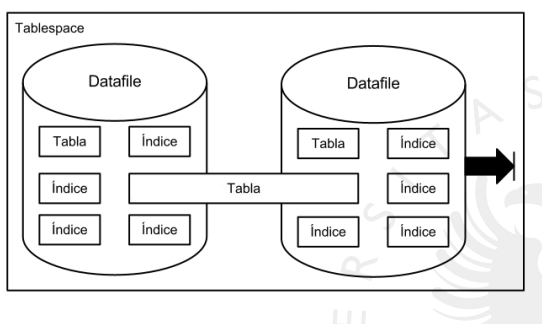
\includegraphics[scale=0.4]{img/12.png}
\end{figure}
\begin{lstlisting}[ language=SQL,
                    deletekeywords={IDENTITY},
                    deletekeywords={[2]INT},
                    morekeywords={clustered},
                    framesep=8pt,
                    xleftmargin=40pt,
                    framexleftmargin=40pt,
                    frame=tb,
                    framerule=0pt ]
ALTER DATABASE DATAFILE "c:\oracle\oradata\users02.dbf" RESIZE 15M;
\end{lstlisting}

Incluso se puede hacer para que el datafile se extienda de forma automática (el uso de \textit{MAXSIZE} se puede omitir, pero es recomendable).

\begin{figure}[H]
  \center
  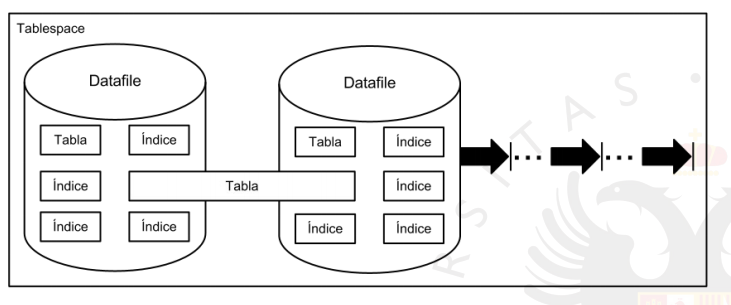
\includegraphics[scale=0.4]{img/13.png}
\end{figure}
\begin{lstlisting}[ language=SQL,
                    deletekeywords={IDENTITY},
                    deletekeywords={[2]INT},
                    morekeywords={clustered},
                    framesep=8pt,
                    xleftmargin=40pt,
                    framexleftmargin=40pt,
                    frame=tb,
                    framerule=0pt ]
ALTER DATABASE DATAFILE "c:\oracle\oradata\users02.dbf" AUTOEXTEND ON NEXT 15M MAXSIZE 100M;
\end{lstlisting}

\subsection{Extensiones, segmentos y bloques}

Internamente, los datafiles almacenan bloques, sin embargo, la forma de estructurar esos bloques no es aleaotria ya que queremos evitar desplazamientos muy largos dentro del disco para poder encontrar rápidamente datos relacionados entre sí. Esa estructura se divide en dos niveles: \textbf{segmentos} y \textbf{extensiones}, de forma que un segmento contiene una serie de extensiones y una extensión contiene una serie de bloques.

Cada vez que se crea una tabla, se crea un segmento que contiene una extensión que contiene un bloque. Es decir, aunque la tabla esté vacía, ocupa espacio (ese bloque). Las extensiones dentro de un segmento se enganchan con punteros y pueden ser de distintos tamaños. Cada extensión contiene un conjunto de bloques. Cuando le extensión se completa, se genera otra extensión encadenada al segmento.

Como al crear el segmento, estamos reservando varios bloques para ese segmento (que no usándolos, ojo) podemos llegar al caso de tener todo el datafile lleno de segmentos, pero con muchos bloques sin usar. ¿Qué pasa si necesitamos crear otro segmento? Se coge un segmento ya existente y se dividen dos si es posible. Luego los segmentos no tienen por qué tener el mismo tamaño.

\begin{figure}[H]
  \center
  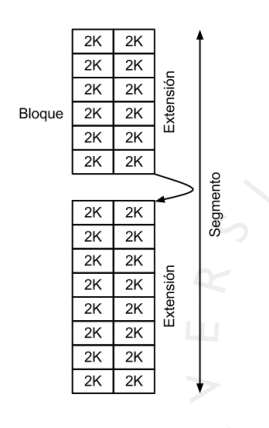
\includegraphics[scale=0.4]{img/14.png}
  \caption{Ejemplo en disco}
\end{figure}

Fijaros que ahí el tamño de las extensiones tampoco es el mismo. ¿Qué tipos de segmentos hay?
\begin{itemize}
\item de datos: tablas
\item de índice: índices
\item temporales: resultados intermedios de \textit{order by}, \textit{group by}, etc. Sobre estos segmentos no hay que almacenar mucha información por eso, porque son temporales y van a desaparecer.
\item de rollback: valores antigusos de datos en \textit{update}. Relacionados con el \textit{redo}, para poder hacer rollback de algunos cambios hechos.
\end{itemize}

Veamos la estructura de un bloque de Oracle:
\begin{itemize}
\item Cabecera: dirección del bloque y tipo de segmento al que está relacionado.
\item Directorio de las tablas que tienen tuplas en el bloque. Cuidado, porque teóricamente lo que hemos visto son los bloques homogéneos, es decir, aquellos bloques que contienen registros de una sola tabla, pero también se pueden contener registros sobre varias tablas en un mismo bloque.
\item Directorio de tuplas del bloque, incluida la dirección. Bastante útil para saltarse tuplas entera (conociendo el offset).
\item Zona de datos donde se almacenan registros. 
\item Espacio libre.
\end{itemize}

\section{Estructura lógica}

El conjunto de objetos de un usuario se denomina \textbf{esquema} y está compuesto por estructuras lógicas como:
\begin{itemize}
\item tablas, vistas, índices, clústers,
\item procedimientos, funciones, paquetes,
\item desparadores, etc.
\end{itemize}
Cada usario tienen un esquema asociado, que tiene el mismo nombre que el usuario al que está relacionado. 

Describamos ahora cada uno de los objetos que puede haber en los esquemas:
\begin{itemize}
\item Tabla: es una estructura lógica con columnas (atributos, identificados por nombre) y filas (tuplas, identificadas por contenido). Al crear una tabla, se crea un segmento con una extensión, y se adjudica a un tablespace por defecto salvo que se especifiquen. Si una fila no cabe en un bloque se genera otro bloque en la extensión, enlazado al anterior, y la tupla se parte.

Cada fila tiene una cabecera con información de cada fragmento, apuntadores, columnas en cada parte, tamaños, etc. Una fila tiene un \textit{rowid} único e invariable. Algunos sistemas admiten el tipo tabla como tipo para una columna.

\begin{example}
Así se crea una tabla asignada al tablespace \textit{users}:
\begin{lstlisting}[ language=SQL,
                    deletekeywords={IDENTITY},
                    deletekeywords={[2]INT},
                    morekeywords={clustered},
                    framesep=8pt,
                    xleftmargin=40pt,
                    framexleftmargin=40pt,
                    frame=tb,
                    framerule=0pt ]
CREATE TABLE CARD ( ... ) TABLESPACE users;
\end{lstlisting}
Recordemos que cada vez que creamos un usuario, se le asigna un tablespace por defecto. Tambíen podemos especificar el tamaño inicial de la extensión ($100K$), el de las siguientes ($100K$) y el número de extensiones máximo que se crearan en el segmento (10):
\begin{lstlisting}[ language=SQL,
                    deletekeywords={IDENTITY},
                    deletekeywords={[2]INT},
                    morekeywords={clustered},
                    framesep=8pt,
                    xleftmargin=40pt,
                    framexleftmargin=40pt,
                    frame=tb,
                    framerule=0pt ]
CREATE TABLE CARD ( ... ) TABLESPACE users 
  STORAGE (INITIAL 100K NEXT 100K MAXEXTENTS 10);
\end{lstlisting}
También podemos eliminar la tabla:
\begin{lstlisting}[ language=SQL,
                    deletekeywords={IDENTITY},
                    deletekeywords={[2]INT},
                    morekeywords={clustered},
                    framesep=8pt,
                    xleftmargin=40pt,
                    framexleftmargin=40pt,
                    frame=tb,
                    framerule=0pt ]
DROP TABLE CARD;
\end{lstlisting}
\end{example}
\item Vista: presentación de datos procedentes de una o más tablas o vistas. Es como guardar una consulta. Se crean mediante el comando \textit{CREATE VIEW}. Para consultar las vistas, se consulta la vista \textit{DBA\_VIEWS}. Básicamente consiste en asignar un nombre a una consulta.

Generalmente, no son actualizables, salvo que se cumplan ciertas restricciones:
\begin{itemize}
\item No pueden incluir agrupadores o agregaciones.
\item No puede incluir la cláusula \textit{DISTINCT}.
\item No puede incluir la reunión ni operadores de conjuntos.
\item Todos los atributos con restricción \textit{NOT NULL} (incluida la clave) deben estar en la vista.
\end{itemize}
Se eliminan mediante la cláusula \textit{DROP VIEW}. ¿Para qué  se usa?
\begin{itemize}
\item Seguridad (ocultar tuplas o atributos)
\item Abstraer de la complejidad de la estructuración de los datos.
\item Simplificar comandos.
\item Aislan aplicaciones de los cambios (si lo que contiene la vista no cambia, claro)
\item Para consultas complejas
\item Para consultas complejas que usan muchos recursos (para no tener que construirlas muchas veces).
\end{itemize}
\item Índice: agilizan el acceso pero ocupan espacio. Enlentecen las inserciones y modificaciones. Hay que pensarlo dos veces antes de crearlos. Oracle crea un índice para la clave (no crees otro). Se usan para:
\begin{itemize}
\item Buscar registros por valores específicos (en columnas indexadas)
\item Recorrer una tabla en orden distinto al físico (ORDER BY)
\item Buscar registros en un rango (en columna indexada)
\end{itemize}
La sentencia para crearlos en \textit{CREATE INDEX}. Después de crear la tabla, mejor insertar las tuplas y después crear al índice (para evitar todas las actualizaciones). La indexación típica suele ser un árbol $B^*$ equilibrado, aunque puede usar bitmaps o hash.
\item Índices multiatributo: índices con más de un atributo son útiles cuando se consulta por los valores de esos atributos de manera ordenada o, en caso de consultarse menos, se consultan desde el primero en adelante. Precisan de mantenimiento, luego deberíamos borrarlos si:
\begin{itemize}
\item Ya no sirven
\item No mejoran la eficiencia
\item Hay que cambiar los campos que se indexan
\item Hay que rehacerlo
\end{itemize}
Para borrarlos se usa la sentencia \textit{DROP INDEX}. Dentro del catálogo se pueden consultar en las tablas \textit{DBA\_INDEXES} y \textit{DBA\_IND\_COLUMNS}.
\item Clusters: para el almacenamiento cercano de tablas que comparten campos y a las que se accede de forma conjunta (reunión natural). Si se accede a cada tabla individualmente y de forma frecuente, no es eficiente. Si se modifican frecuentemente las tablas (en tuplas) no es eficiente. Mejoran la reunión natural al reducir los accesos a disco. El campo o campos de reunión natural se almacenan una sola vez (claro ejemplo de bloques heterogéneos). ¿Cómo se crea? Primero se crea con \textit{CREATE CLUSTER}. Luego hay que crear las tablas del cluster:
\begin{lstlisting}[ language=SQL,
                    deletekeywords={IDENTITY},
                    deletekeywords={[2]INT},
                    morekeywords={clustered},
                    framesep=8pt,
                    xleftmargin=40pt,
                    framexleftmargin=40pt,
                    frame=tb,
                    framerule=0pt ]
CREATE TABLE <nombre> (
  ...
) CLUSTER <nombre> (<campos de reunion>);
\end{lstlisting}
Antes de insertar datos, crear el índice sobre los campos del clúster:
\begin{lstlisting}[ language=SQL,
                    deletekeywords={IDENTITY},
                    deletekeywords={[2]INT},
                    morekeywords={clustered},
                    framesep=8pt,
                    xleftmargin=40pt,
                    framexleftmargin=40pt,
                    frame=tb,
                    framerule=0pt ]
CREATE INDEX <nombre> ON CLUSTER <nombre>;
\end{lstlisting}
Puede borrarse con la sentencia \textit{DROP CLUSTER}, pero primero hay que borrar las tablas de dentro, o usar la sentencia \textit{INCLUDING TABLES}. También hay que borrar las llaves externas que las referencian salvo que se incluya la sentencia \textit{CASCADE CONSTRAINTS}. Se puede borrar su índice con \textit{DROP INDEX} pero no se podrá acceder al contenido del clúster si no se reconstruye dicho índice.
\end{itemize}